% All contribution chapters should follow a similar structure, with a
% mini-introduction and overview at the beginning and a conclusion at the
% end bookmarking a structured presentation of the contribution. This can be
% largely based on your publications.

\chapter{Simulation of Biofilm Development}\label{chap:contrib3}

\section{Progression of a Simulated Biofilm Monolayer}

We present the sequential development of a simulated biofilm monolayer. We will analyze the evolution of the cytoplasmic proteins involved in the gene regulatory network and the development of phenotypes at 1-hour intervals, starting from the 4th hour after inoculation.

\subsection{After 4 Hours}\label{sec:contrib3:theme1}

During the first 4 hours of the simulation, the initial cells, commonly known as pioneer cells, initiate the process of biofilm formation. This group of cells consists exclusively of undifferentiated cells (Figure 5.1). The initial group of cells secretes the ComX pheromone, which rapidly diffuses across the grid of pixels in all directions. According to our model, each bacterium produces the ComX pheromone constitutively, regardless of its phenotype or environmental conditions. The continuous production of the ComX pheromone makes it an effective indicator of cell density. At this stage of biofilm development, no cells express the surfactin-producing phenotype, resulting in a complete absence of surfactin in the extracellular space.

At this point, the concentration of SinR molecules in every cell exceeds 75 nM. This is due to the absence of SinI or SlrR molecules for binding, and the production rate of SinR \(P_3\) is greater than the dilution rate caused by cell growth and degradation \(D_{R}\). Conversely, the concentration of SinI and SlrR is very low. The absence of SinI molecules at this stage is due to the absence of surfactin in the environment, which is necessary to stimulate SinI transcription. The absence of SlrR molecules is due to the high concentration of SinR, which strongly inhibits the expression of SlrR.

\begin{figure}[h]
    \centering
    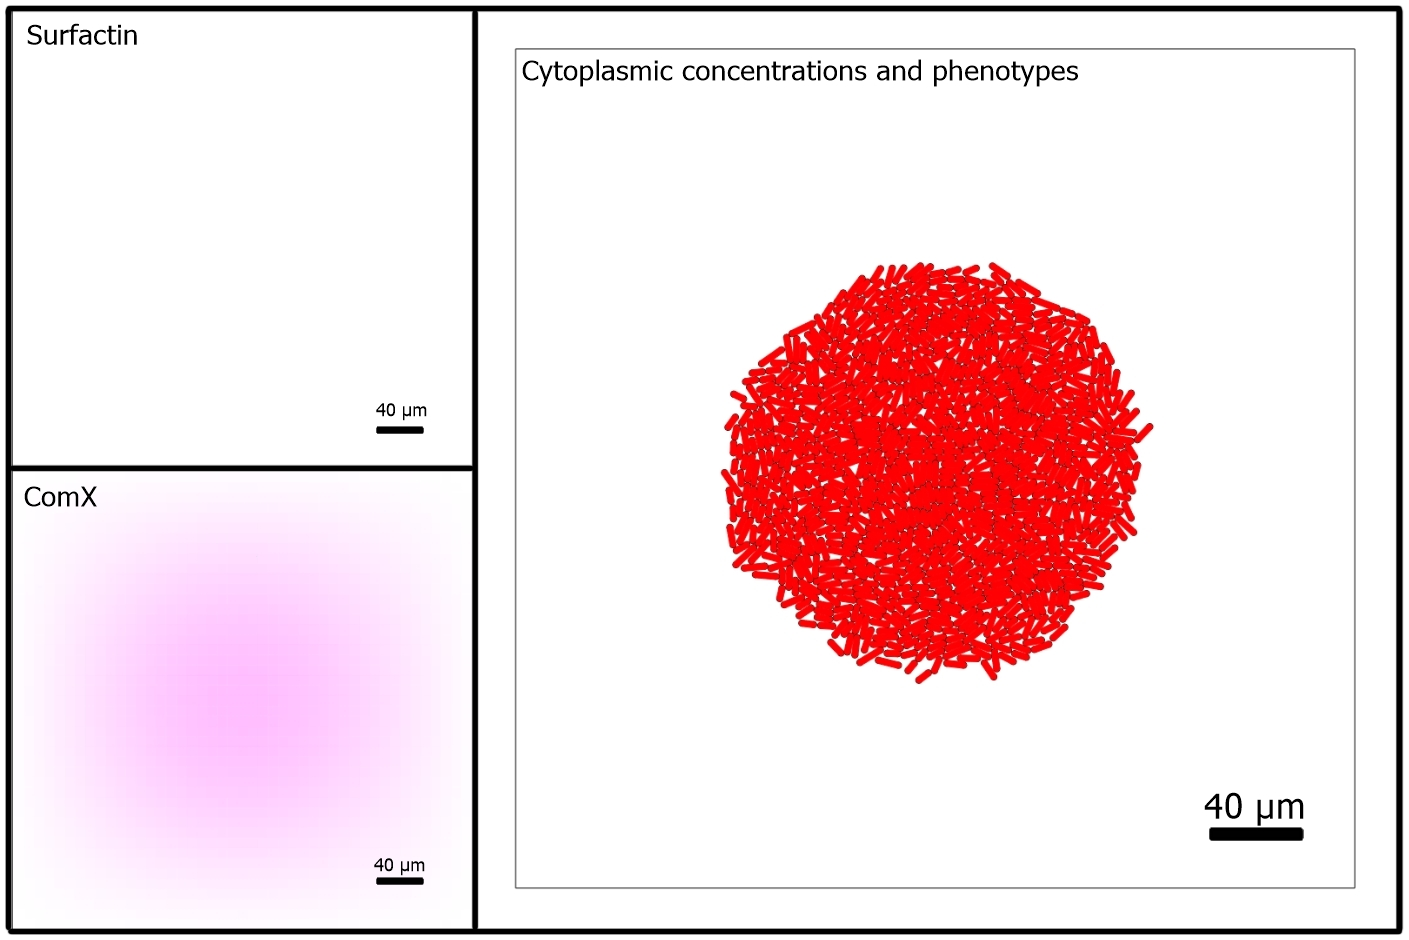
\includegraphics[width=0.98\textwidth]{Final_run4.jpg}
    \caption{\footnotesize \textbf{Extracellular and intracellular concentrations of signaling molecules and gene regulatory proteins 4 hours after inoculation.} The image in the top-left corner shows the extracellular concentration of surfactin across the biofilm, which, at this stage of development, is zero. The image in the bottom left corner shows the extracellular concentration of ComX across the biofilm, measured in arbitrary units. The intracellular concentrations of SinR, SinI, and SlrR are represented as a point in the three-dimensional red-green-blue additive color space. Specifically, SinR concentration is mapped to the red channel, SinI to the green channel, and SlrR to the blue channel. Since all cells have a high concentration of SinR and a low concentration of SinI and SlrR, they all appear 100\% red.}


\end{figure}

\begin{figure}[h]
    \centering
    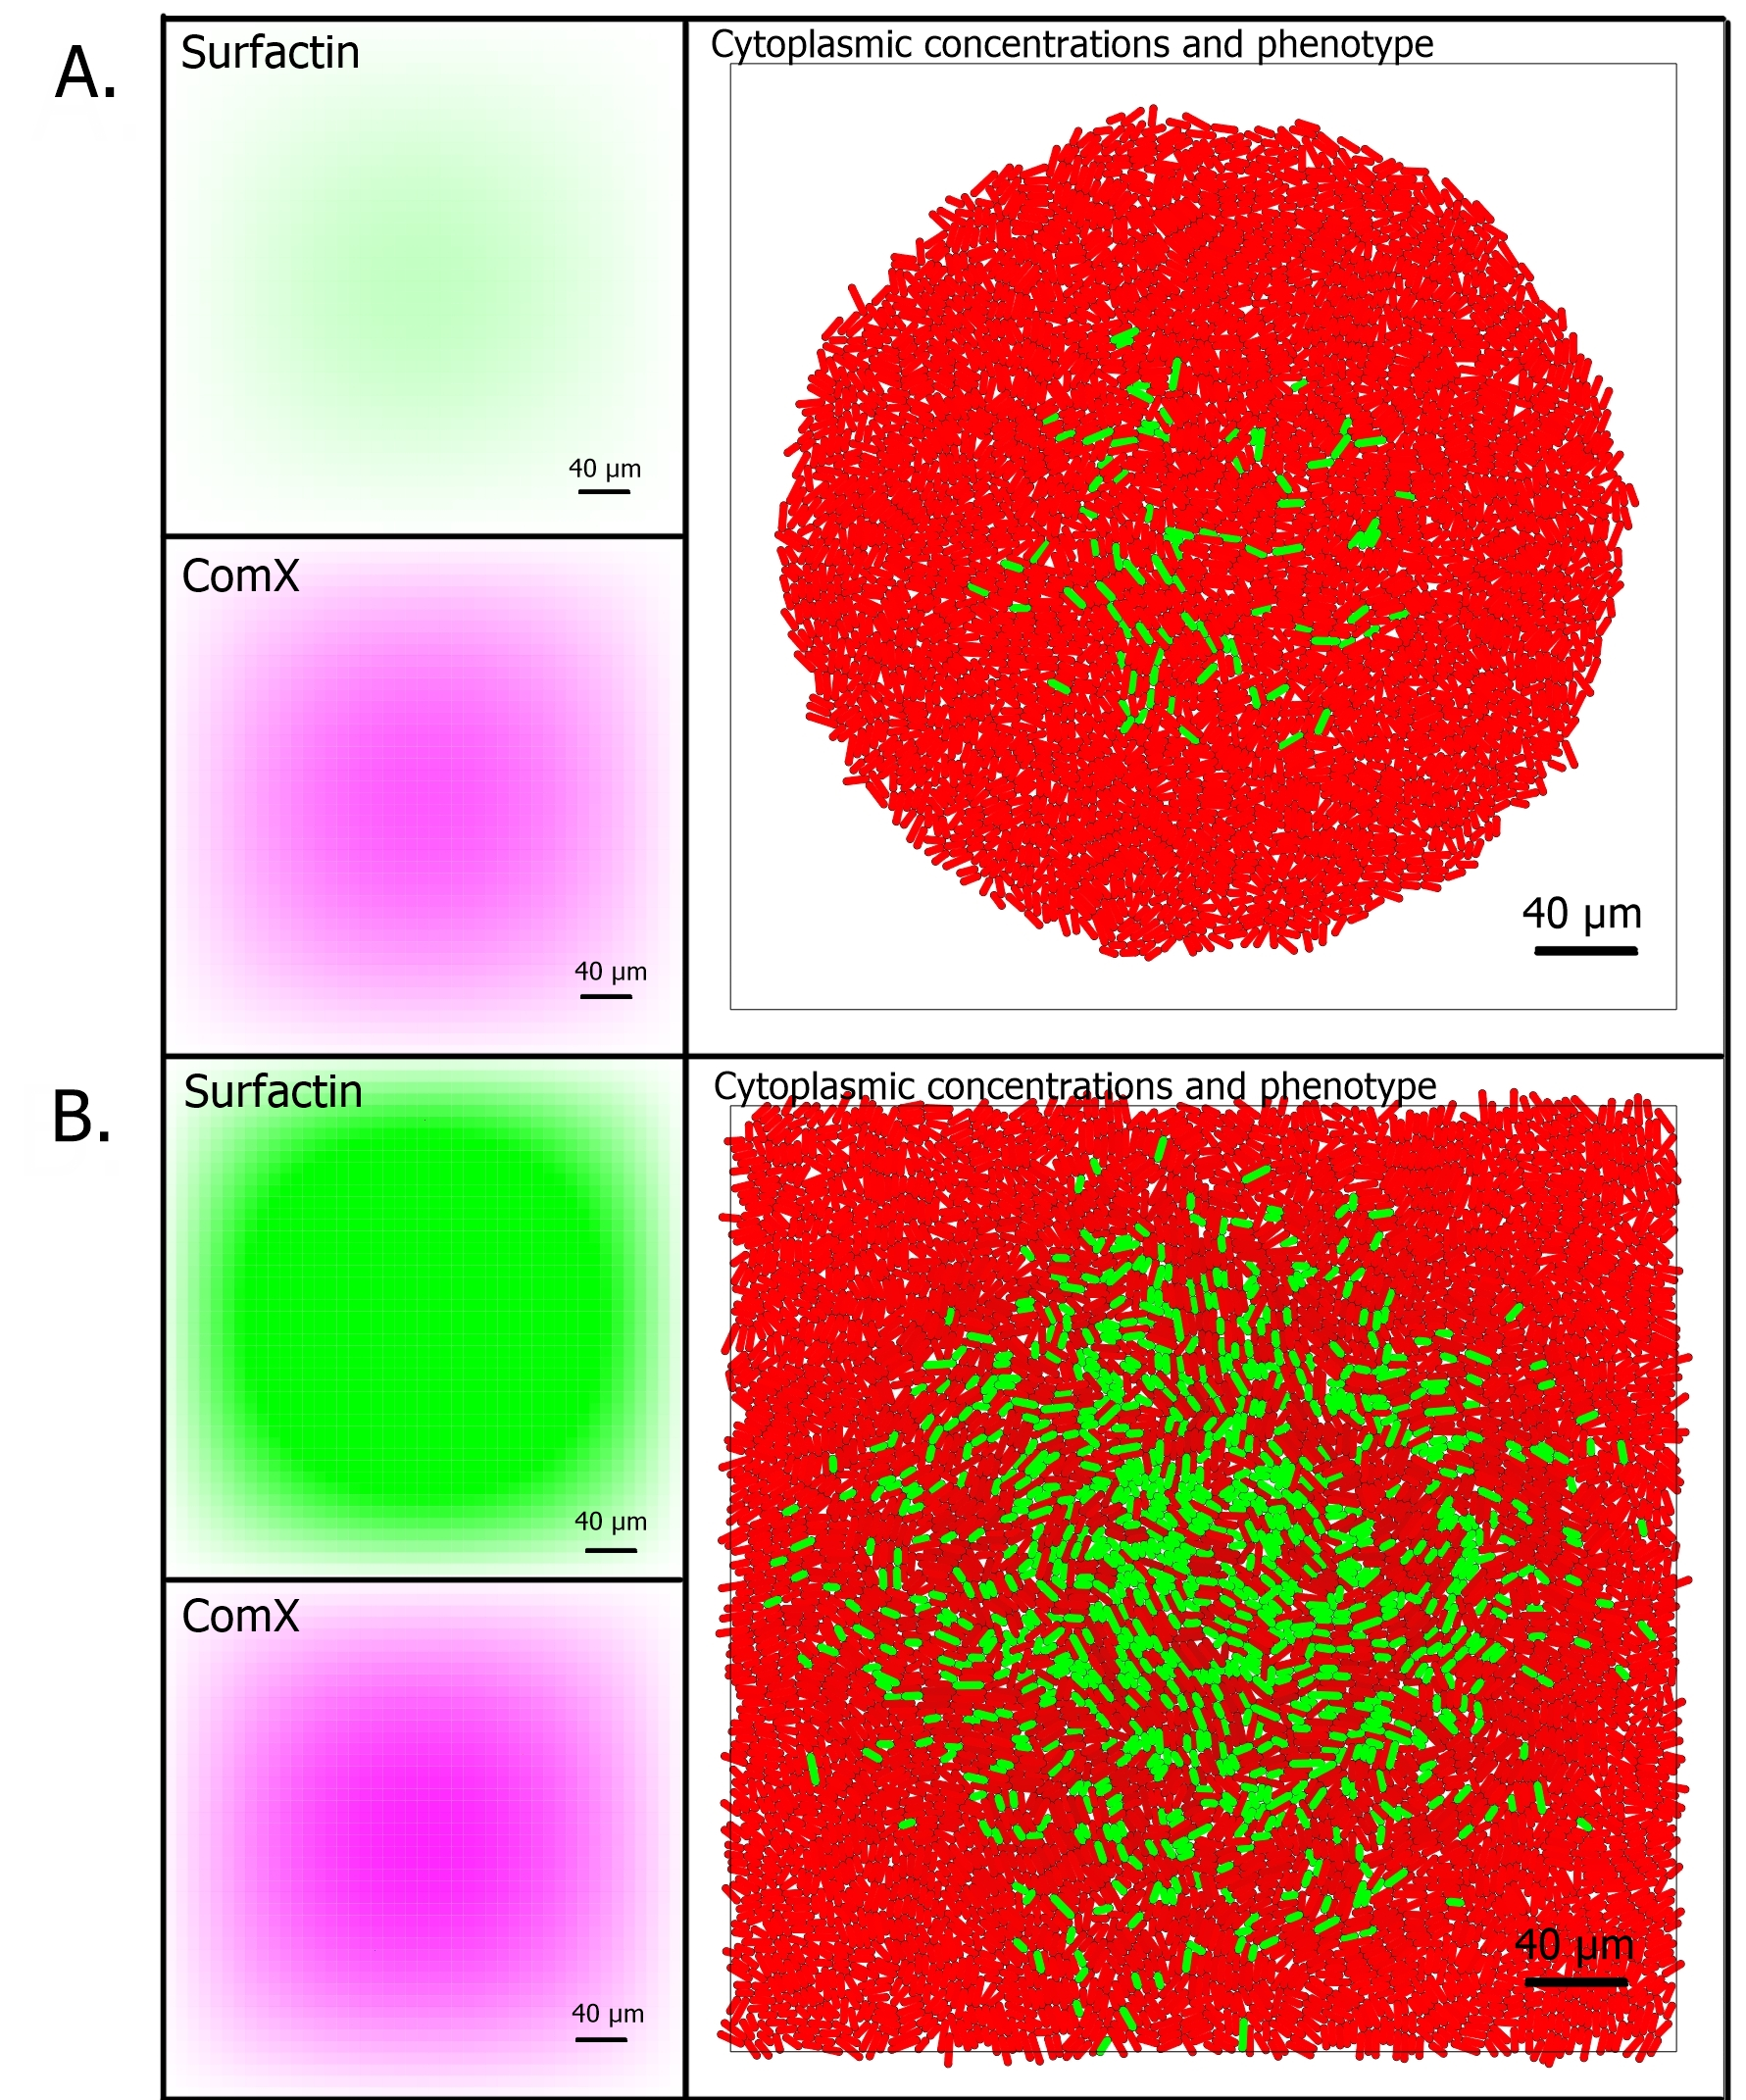
\includegraphics[width=0.98\textwidth]{Final_run2.jpg}
    \caption{\footnotesize \textbf{Extracellular and intracellular concentrations of signaling molecules and gene regulatory proteins 5 and 6 hours after inoculation.} A. Shows the simulation's state after 5 hours. B. Shows the simulation's state after 6 hours. The images in the top-left corners of A and B show the extracellular concentration of surfactin across the biofilm in green, measured in arbitrary units. The images in the bottom left corners of A and B show the extracellular concentration of ComX across the biofilm in pink, measured in arbitrary units. On the right side of A and B, the surfactin producers are shown in green. The intracellular concentrations of SinR, SinI, and SlrR of the non-surfactin-producing cells are represented as a point in the three-dimensional red-green-blue additive color space. Specifically, the SinR concentration is mapped to the red channel, SinI to the green channel, and SlrR to the blue channel. Since all cells have a high concentration of SinR and a low concentration of SinI and SlrR, they all appear almost 100\% red. }


\end{figure}

\subsection{After 5 and 6 Hours}\label{sec:contrib3:theme1}
As the cell population grows, the concentration of the ComX pheromone increases throughout the entire two-dimensional space, particularly in the central region of the biofilm. An elevated extracellular concentration of this pheromone triggers the expression of the surfactin-producing phenotype in cells that are particularly sensitive to ComX. At this stage, we can observe that a certain amount of surfactin has accumulated in the extracellular space. However, the concentration of surfactin is not high enough to cause any significant alteration in the bacterial cytoplasmic state. The total number of intracellular regulatory proteins remains almost unchanged compared to the concentration observed at the 4th hour (see Figure 5.2.A).

At the 6th hour, we observed a significant increase in the number of cells producing surfactin, as well as a rise in the concentration of extracellular surfactin (see Figure 5.2.B). If we observe carefully, we can also notice a slight decrease in the intensity of the red color in cells located at the center of the biofilm. This indicates a slight decrease in the concentration of SinR.


\begin{figure}[h]
    \centering
    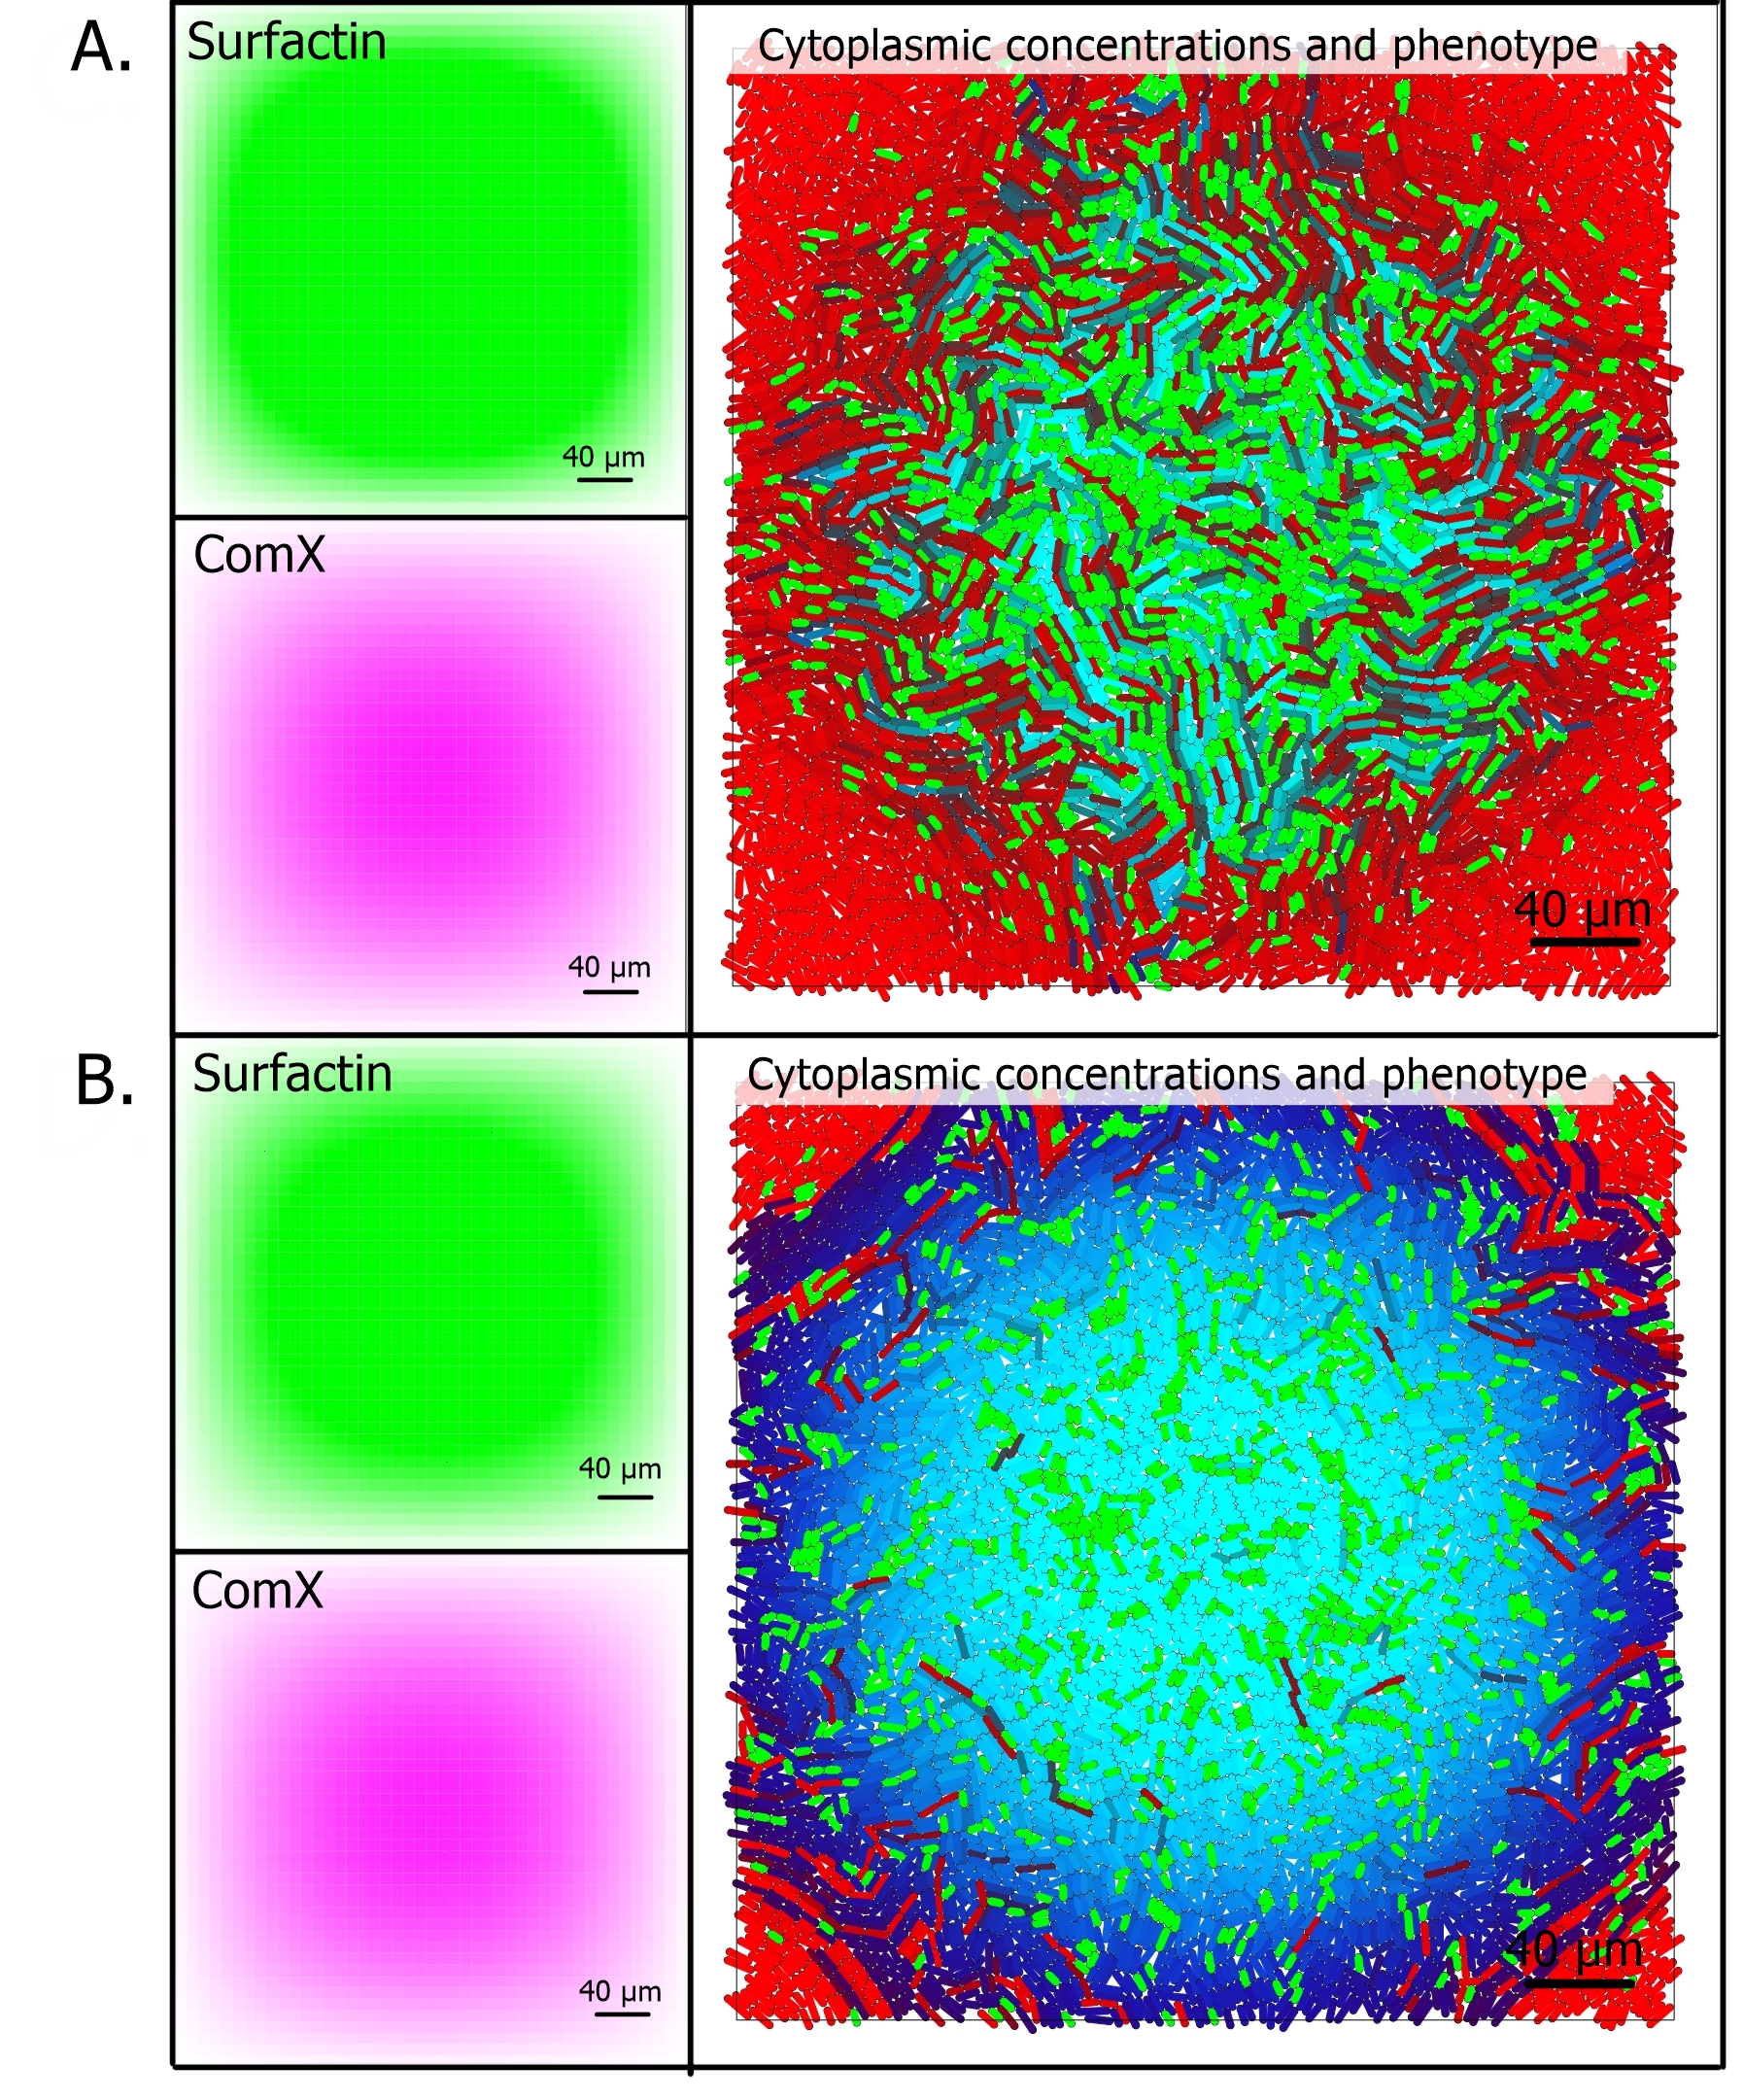
\includegraphics[width=0.98\textwidth]{Final_run3.jpg}
        \caption{\footnotesize \textbf{Extracellular and intracellular concentrations of signaling molecules and gene regulatory proteins 7 and 8 hours after inoculation.} A. Shows the simulation's state after 7 hours. B. Shows the simulation's state after 8 hours. The images in the top-left corners of A and B show the extracellular concentration of surfactin across the biofilm in green, measured in arbitrary units. The images in the bottom left corners of A and B show the extracellular concentration of ComX across the biofilm in pink, measured in arbitrary units. On the right side of A and B, the surfactin producers are shown in green. The intracellular concentrations of SinR, SinI, and SlrR of the non-surfactin-producing cells are represented as a point in the three-dimensional red-green-blue additive color space. Specifically, the SinR concentration is mapped to the red channel, SinI to the green channel, and SlrR to the blue channel. This way, cells with a high concentration of only SinR appear red. Cells with a high concentration of only SlrR appear blue. Cells with a high concentration of both SlrR and SinI appear in cyan. There are no cells that have only a high concentration of SinI.}

\end{figure}
\subsection{After 7 and 8 Hours}\label{sec:contrib3:theme1}

After 7 hours, a high concentration of surfactin activates the transcription of SinI, thereby increasing the concentration of SinI molecules in the cytoplasm. The SinI protein binds to SinR, forming a complex that effectively reduces the number of available SinR molecules in the cytoplasm. This is the reason for the significant decrease in the concentration of SinR in cells situated at the center of the biofilm. At the same time, we observe an increase in the concentration of SlrR, particularly in cells located near the center of the biofilm. This happens when the concentration of SinR drops below a threshold at which it becomes ineffective in inhibiting the expression of SlrR. (Figure 5.3.A)

At this stage, we can observe that many of the cells at the center of the biofilm have a very low concentration of SinR, which allows for the activation of the matrix production phenotype. This phenotype has the unique characteristic of being insensitive to ComX. This implies that as long as the bacteria continue to produce extracellular matrix, they will be unable to sense ComX and will not activate the surfactin-producing phenotype. In this scenario, if the majority of cells in the simulation are matrix producers and they continue to grow and reproduce, they will push the surfactin producers outside the simulation area. Over time, the biofilm will eventually displace its entire population of surfactin-producing cells, which are unable to grow and reproduce. (Figure 5.3.B)

As a result, a decrease in the concentration of surfactin will lead to a reduction in the production of SinI. Because of that, there will be an increase in the concentration of SinR, which will ultimately inhibit matrix production. The described phenomenon leads to oscillatory behavior in the composition of phenotypes. (Figures 5.5)

\begin{figure}[h]
    \centering
    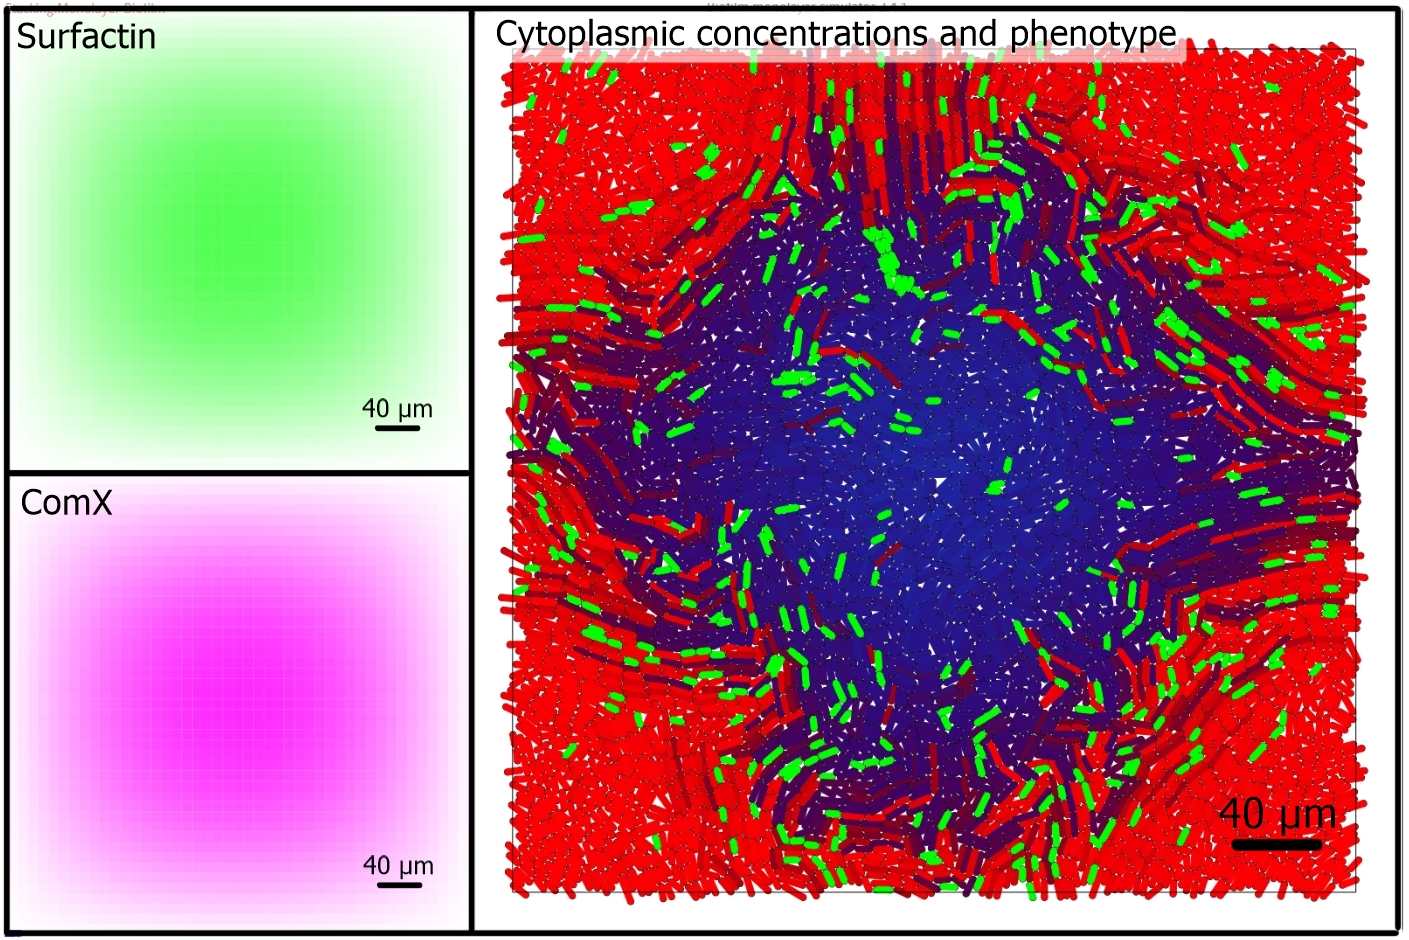
\includegraphics[width=0.98\textwidth]{elfin.jpg}
    \caption{\footnotesize \textbf{Extracellular and intracellular concentrations of signaling molecules and gene regulatory proteins 12 hours after inoculation.} The image in the top-left corner shows the extracellular concentration of surfactin across the biofilm in green, measured in arbitrary units. The image in the bottom left corner show the extracellular concentration of ComX across the biofilm in pink, measured in arbitrary units. On the right, the surfactin producers are shown in green. The intracellular concentrations of SinR, SinI, and SlrR of the non-surfactin-producing cells are represented as a point in the three-dimensional red-green-blue additive color space. Specifically, the SinR concentration is mapped to the red channel, SinI to the green channel, and SlrR to the blue channel. This way, cells with a high concentration of only SinR appear red. Cells with a high concentration of only SlrR appear in Blue. There are no cells that have only a high concentration of SinI.}



\end{figure}

\subsection{After 12 Hours}\label{sec:contrib3:theme1}

At this stage, we can observe that in many cells, the concentration of SinI and SlrR has decreased, while the concentration of SinR has increased, compared to the state after 8 hours. (See Figure 5.4). This indicates that the transition from high-SinR to low-SinR concentration is not permanent, but rather it continues to evolve as the concentration of surfactin decreases in the environment.


\clearpage

\section{Phenotype oscillations}
When plotting the number of cells exhibiting each phenotype, it becomes evident that the composition of phenotypes continues to oscilate as time increases.

In Figure 5.5, we can observe that the number of bacteria producing the matrix has reached its peak at approximately the 9th hour. At this time step, most cells are resistant to ComX due to the presence of the extracellular matrix. No matter how high the concentration of ComX is, it cannot activate the surfactin-producing phenotype in most cells. At the same time, undifferentiated cells and matrix-producing cells continue to grow and reproduce, displacing the few existing surfactin producers out of the simulation area. This causes a drop in surfactin producers at around the 10th hour. Upon examining the development of the biofilm within the first 20 hours (Figure 5.5), it becomes apparent that the composition of phenotypes continues to oscillate, showing no signs of equilibrium.

\begin{figure}[h]
    \centering
    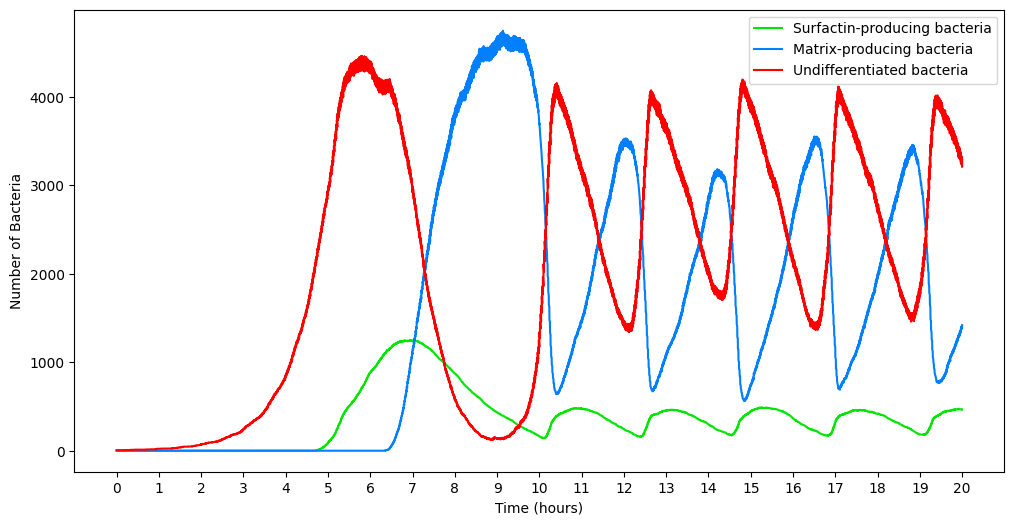
\includegraphics[width=1\textwidth]{phenotype_short.png}
    \caption{\footnotesize \textbf{Count of cell phenotypes throughout the simulation.} The quantities of matrix producers, surfactin producers, and undifferentiated cells are shown on the left axis. The maximum number of cells allowed at any given time is approximately 5200 bacteria.}


    
\end{figure} 

 



%\section{Minute 300th}\label{sec:contrib3:theme1}

%\begin{figure}[h]
  %  \centering
   % \includegraphics[width=1\textwidth]{300_minutes}
 %   \caption{\textbf{Extracellular and intracellular concentrations of signaling molecules and gene regulatory proteins 300 minutes after inoculation.} The top-left image in the diagram displays the color-coded cell phenotype, as well as the extracellular concentration of ComX. Cells with an undifferentiated phenotype are represented in pink, cells expressing the surfactin-producing phenotype are represented in green, and cells expressing the matrix producing phenotype are represented in blue. The extracellular ComX concentration is represented by a pink gradient in the background and is measured in arbitrary units. The images in the top-right, bottom-left, and bottom-right show the cytoplasmic counts of SinR, SinI, and SlrR molecules within individual cells. The scale ranges from black, indicating zero molecules, to white, indicating 85 or more molecules. These last three images also illustrate the concentration of extracellular surfactin, depicted as a green gradient in the background. The concentration of surfactin is measured in arbitrary units.}
    
%\end{figure}
\clearpage



\section{Conclusion}

In this chapter, we presented the sequential development of a simulated biofilm monolayer. We analyzed the evolution of the cytoplasmic proteins involved in the gene regulatory network and gave a detailed explanation and interpretation of the development of phenotypes. In the next chapter, we will present the conclusions of this thesis and discuss the future work and possible applications of the model.
